%%%%%%%%%%%%%%%%%%%%%%%%%%%%%%%%%%%%%%%%%
% Programming/Coding Assignment
% LaTeX Template
%
% This template has been downloaded from:
% http://www.latextemplates.com
%
% Original author:
% Ted Pavlic (http://www.tedpavlic.com)
%
% Note:
% The \lipsum[#] commands throughout this template generate dummy text
% to fill the template out. These commands should all be removed when 
% writing assignment content.
%
% This template uses a Perl script as an example snippet of code, most other
% languages are also usable. Configure them in the "CODE INCLUSION 
% CONFIGURATION" section.
%
%%%%%%%%%%%%%%%%%%%%%%%%%%%%%%%%%%%%%%%%%

%----------------------------------------------------------------------------------------
%	PACKAGES AND OTHER DOCUMENT CONFIGURATIONS
%----------------------------------------------------------------------------------------

\documentclass{article}

\usepackage{fancyhdr} % Required for custom headers
\usepackage{lastpage} % Required to determine the last page for the footer
\usepackage{extramarks} % Required for headers and footers
\usepackage[usenames,dvipsnames]{color} % Required for custom colors
\usepackage{graphicx} % Required to insert images
\usepackage{listings} % Required for insertion of code
\usepackage{courier} % Required for the courier font
\usepackage{lipsum} % Used for inserting dummy 'Lorem ipsum' text into the template
\usepackage[utf8]{inputenc}
\usepackage[ngerman]{babel}
\usepackage{minted}

% Margins
\topmargin=-0.45in
\evensidemargin=0in
\oddsidemargin=0in
\textwidth=6.5in
\textheight=9.0in
\headsep=0.25in

\linespread{1.1} % Line spacing

% Set up the header and footer
\pagestyle{fancy}
%\lhead{\hmwkAuthorName} % Top left header
\chead{\hmwkClass\ : \hmwkTitle} % Top center head
\rhead{\firstxmark} % Top right header
\lfoot{\lastxmark} % Bottom left footer
\cfoot{} % Bottom center footer
\rfoot{Page\ \thepage\ of\ \protect\pageref{LastPage}} % Bottom right footer
\renewcommand\headrulewidth{0.4pt} % Size of the header rule
\renewcommand\footrulewidth{0.4pt} % Size of the footer rule

\setlength\parindent{0pt} % Removes all indentation from paragraphs

%----------------------------------------------------------------------------------------
%	CODE INCLUSION CONFIGURATION
%----------------------------------------------------------------------------------------

\definecolor{MyDarkGreen}{rgb}{0.0,0.4,0.0} % This is the color used for comments
\lstloadlanguages{Perl} % Load Perl syntax for listings, for a list of other languages supported see: ftp://ftp.tex.ac.uk/tex-archive/macros/latex/contrib/listings/listings.pdf
\lstset{language=Perl, % Use Perl in this example
        frame=single, % Single frame around code
        basicstyle=\small\ttfamily, % Use small true type font
        keywordstyle=[1]\color{Blue}\bf, % Perl functions bold and blue
        keywordstyle=[2]\color{Purple}, % Perl function arguments purple
        keywordstyle=[3]\color{Blue}\underbar, % Custom functions underlined and blue
        identifierstyle=, % Nothing special about identifiers                                         
        commentstyle=\usefont{T1}{pcr}{m}{sl}\color{MyDarkGreen}\small, % Comments small dark green courier font
        stringstyle=\color{Purple}, % Strings are purple
        showstringspaces=false, % Don't put marks in string spaces
        tabsize=5, % 5 spaces per tab
        %
        % Put standard Perl functions not included in the default language here
        morekeywords={rand},
        %
        % Put Perl function parameters here
        morekeywords=[2]{on, off, interp},
        %
        % Put user defined functions here
        morekeywords=[3]{test},
       	%
        morecomment=[l][\color{Blue}]{...}, % Line continuation (...) like blue comment
        numbers=left, % Line numbers on left
        firstnumber=1, % Line numbers start with line 1
        numberstyle=\tiny\color{Blue}, % Line numbers are blue and small
        stepnumber=5 % Line numbers go in steps of 5
}

% Creates a new command to include a perl script, the first parameter is the filename of the script (without .pl), the second parameter is the caption
\newcommand{\perlscript}[2]{
\begin{itemize}
\item[]\lstinputlisting[caption=#2,label=#1]{#1.pl}
\end{itemize}
}

%----------------------------------------------------------------------------------------
%	DOCUMENT STRUCTURE COMMANDS
%	Skip this unless you know what you're doing
%----------------------------------------------------------------------------------------

% Header and footer for when a page split occurs within a problem environment
\newcommand{\enterProblemHeader}[1]{
%\nobreak\extramarks{#1}{#1 continued on next page\ldots}\nobreak
%\nobreak\extramarks{#1 (continued)}{#1 continued on next page\ldots}\nobreak
}

% Header and footer for when a page split occurs between problem environments
\newcommand{\exitProblemHeader}[1]{
%\nobreak\extramarks{#1 (continued)}{#1 continued on next page\ldots}\nobreak
%\nobreak\extramarks{#1}{}\nobreak
}

\setcounter{secnumdepth}{0} % Removes default section numbers
\newcounter{homeworkProblemCounter} % Creates a counter to keep track of the number of problems

\newcommand{\homeworkProblemName}{}
\newenvironment{homeworkProblem}[1][Problem \arabic{homeworkProblemCounter}]{ % Makes a new environment called homeworkProblem which takes 1 argument (custom name) but the default is "Problem #"
\stepcounter{homeworkProblemCounter} % Increase counter for number of problems
\renewcommand{\homeworkProblemName}{#1} % Assign \homeworkProblemName the name of the problem
\section{\homeworkProblemName} % Make a section in the document with the custom problem count
\enterProblemHeader{\homeworkProblemName} % Header and footer within the environment
}{
\exitProblemHeader{\homeworkProblemName} % Header and footer after the environment
}

\newcommand{\problemAnswer}[1]{ % Defines the problem answer command with the content as the only argument
\noindent\framebox[\columnwidth][c]{\begin{minipage}{0.98\columnwidth}#1\end{minipage}} % Makes the box around the problem answer and puts the content inside
}

\newcommand{\homeworkSectionName}{}
\newenvironment{homeworkSection}[1]{ % New environment for sections within homework problems, takes 1 argument - the name of the section
\renewcommand{\homeworkSectionName}{#1} % Assign \homeworkSectionName to the name of the section from the environment argument
\subsection{\homeworkSectionName} % Make a subsection with the custom name of the subsection
\enterProblemHeader{\homeworkProblemName\ [\homeworkSectionName]} % Header and footer within the environment
}{
\enterProblemHeader{\homeworkProblemName} % Header and footer after the environment
}

%----------------------------------------------------------------------------------------
%	NAME AND CLASS SECTION
%----------------------------------------------------------------------------------------

\newcommand{\hmwkTitle}{Übung\ \#2} % Assignment title
\newcommand{\hmwkDueDate}{Montag,\ 03.\ November\ 2014} % Due date
\newcommand{\hmwkClass}{Reconfigurable Embedded Systems} % Course/class
\newcommand{\hmwkClassTime}{} % Class/lecture time
\newcommand{\hmwkClassInstructor}{} % Teacher/lecturer
\newcommand{\hmwkAuthorName}{Günther Schindler, Sven Dorkenwald} % Your name

%----------------------------------------------------------------------------------------
%	TITLE PAGE
%----------------------------------------------------------------------------------------

\title{
\vspace{2in}
\textmd{\textbf{\hmwkClass:\ \hmwkTitle}}\\
\normalsize\vspace{0.1in}\small{Abgabe\ am\ \hmwkDueDate}\\
\vspace{0.1in}\large{\textit{\hmwkClassTime}}
\vspace{3in}
}

\author{\textbf{\hmwkAuthorName}}
\date{} % Insert date here if you want it to appear below your name

%----------------------------------------------------------------------------------------

\begin{document}

\maketitle

%----------------------------------------------------------------------------------------
%	TABLE OF CONTENTS
%----------------------------------------------------------------------------------------

%\setcounter{tocdepth}{1} % Uncomment this line if you don't want subsections listed in the ToC

\newpage
\tableofcontents
\newpage

%----------------------------------------------------------------------------------------
%	PROBLEM 1
%----------------------------------------------------------------------------------------

% To have just one problem per page, simply put a \clearpage after each problem

\begin{homeworkProblem}[Seriell-Parallel-Wandler]
Folgender VHDL-Code (SP\_Decoder) beschreibt das Verhalten eines Seriell-Parallel-Wandlers. 
Ein Eingangssignal (din) wird taktweise eingelesen und auf vier Ausgangssignale 
(LED\_REG) nach dem vierten Takt geschaltet. Realisiert wurde dieses Schieberegister
mit einer Finite State Machine (FSM) mit vier Zuständen (S0-S4). Der asynchrone 
Reset setzt die Ausgangssignale sofort auf '0000' und die FSM in den Grundzustand S0.
\begin{minted}{vhdl}
library IEEE;
use IEEE.STD_LOGIC_1164.ALL;

entity SP_Decoder is
port( clk, reset, din: in std_logic; LED_REG: out std_logic_vector(3 downto 0));
end SP_Decoder;

architecture Behavioral of SP_Decoder is
signal INT_REG: std_logic_vector(3 downto 0) := (others => '0');
type states is (S0, S1, S2, S3);
signal state: states := S0;
begin
  process(clk, reset)
  begin
    if reset = '1' then 
      INT_REG <= (others => '0');
      LED_REG <= (others => '0');
      state <= S0;
    elsif rising_edge(clk) then
    case state is
      when S0 =>
	LED_REG <= INT_REG;
	INT_REG <=  INT_REG(2 downto 0) & din;
	state <= S1;
      when S1 =>
	INT_REG <= INT_REG(2 downto 0) & din;
	state <= S2;
      when S2 =>
	INT_REG <= INT_REG(2 downto 0) & din;
	state <= S3;
      when S3 =>
	INT_REG <= INT_REG(2 downto 0) & din;
	state <= S0;
    end case;
    end if;
  end process;
end Behavioral;
\end{minted}
Die zugehörige Testbench ("tb\_SP\_Decoder") simuliert hintereinander die drei 
Bitsequenzen '1101', '1001' und '0101'. Zur Synchronistation verwendet die 
Testbench den asynchronen Reset.
\\\\
Die Prozedur "clk\_procedure" wird eingesetzt um einen freilaufenden Takt zu
vermeiden. Sie invertiert den Takt und wartet eine halbe Taktperiode (5 ns).
\begin{minted}{vhdl}
...
procedure clk_procedure(
  signal clk_IN: in std_logic;
  signal clk_OUT: out std_logic
)is
begin
  clk_OUT <= not clk_IN;
  wait for clk_period/2;
end clk_procedure;
...
\end{minted}
Im Impulsprozess (stim\_proc) wird durch zweimaligen Aufruf der clk\_procedure
ein Taktimpuls simuliert. Bitweiße werden die Testsequenzen durch din eingelesen.
Ist jeweils die 4-Bit-Sequenz eingelesen und der vierte Taktzyklus vollendet,
wird mit der assert-Anweisung das Ausgangssignal LED\_REG überprüft und eine
Ausgabe an die Standardausgabe vorgenommen.
\begin{minted}{vhdl}
...
stim_proc: process
  begin
    reset <= '1';
      clk_procedure(clk,clk);
      clk_procedure(clk,clk);
      reset <= '0';
      -- first sequenz: 1101
      assert false report "INFO: Starting sequence '1101'" severity note;
      din <= '1';
      clk_procedure(clk,clk);
      clk_procedure(clk,clk);
      din <= '1';
      clk_procedure(clk,clk);
      clk_procedure(clk,clk);
      din <= '0';
      clk_procedure(clk,clk);
      clk_procedure(clk,clk);
      din <= '1';
      clk_procedure(clk,clk);
      clk_procedure(clk,clk);
      -- second sequenz: 1001
      din <= '1';
      clk_procedure(clk,clk);
      assert (LED_REG = "1101") report "ERROR: Output is not equal '1101', failure!" severity error;
      assert (LED_REG /= "1101") report "INFO: Output is equal '1101', ok!" severity note;
      assert false report "INFO: Starting sequence '1001'" severity note;
		
      ...
		
      wait;
end process;
\end{minted}
Die analyse der Waveform bestätigt das korrekte Verhalten des Seriell-Parallel-Wandlers. Nachdem der reset auf '0' gesetzt wird, werden bitweise die Signale
auf die Eingangsleitung (din) übertragen. Nach dem vierten Taktzyklus (angefangen ab der ersten steigenden Flanke nachdem reset = '0') wird das Signal '1101' auf die Ausgangssignalleitung
(LED\_REG) geschaltet. Nach jeweils weiteren vier Taktzyklen wird LED\_REG '1001' und danach '0101'. 
\begin{center}
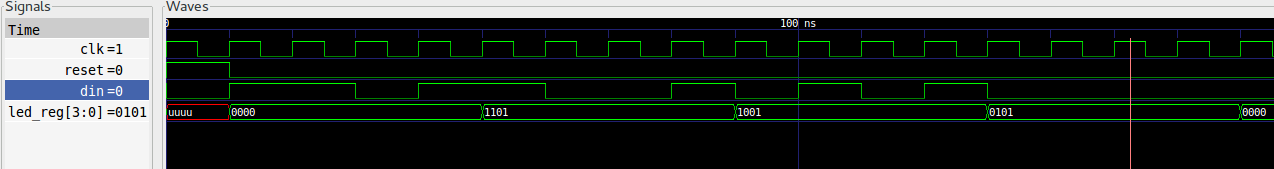
\includegraphics[width=1\columnwidth]{SP_Sim}
\end{center}
Auch die assertion-Ausgaben der Testbench bestätigen das korrekte Verhalten.
\begin{center}
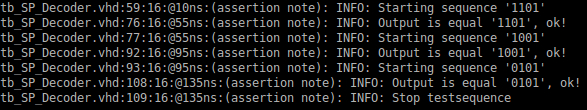
\includegraphics[width=0.5\columnwidth]{Output}
\end{center}
\end{homeworkProblem}
%Listing \ref{homework_example} shows a Perl script.

%\perlscript{homework_example}{Sample Perl Script With Highlighting}

%\lipsum[1]

%----------------------------------------------------------------------------------------
%	PROBLEM 2
%----------------------------------------------------------------------------------------

\begin{homeworkProblem}[4-Bit-Multiplexer]
Folgender VHDL-Quellcode (MUX) zeigt eine Implementierung eines 4-input Multiplexers, 
basierend auf einer Look-up-table (LUT).

\begin{minted}{vhdl}
library IEEE;
use IEEE.STD_LOGIC_1164.ALL;

entity MUX is
port(D3, D2, D1, D0: in std_logic; SEL: in std_logic_vector(1 downto 0); Y: out std_logic);
end MUX;

architecture Behavioral of MUX is
begin
  process(SEL, D3, D2, D1, D0)
  begin
    case SEL is
      when "00" => Y <= D0;
      when "01" => Y <= D1;
      when "10" => Y <= D2;
      when "11" => Y <= D3;
      when others => NULL;
    end case;
  end process;
end Behavioral;
\end{minted}
Die Testbench (tb\_MUX) des Multiplexers prüft alle möglichen Kombinationen von 
Datensignale (D3 - D0) und Steuersignal (SEL).
\\\\
Um die Steuersignale zu variieren wird die Prozedur p\_inc\_slv verwendet, welche 
die übergeben Adresse inkrementiert. 
\begin{minted}{vhdl}
procedure p_inc_slv (
  signal r_IN: in std_logic_vector(1 downto 0);
  signal r_OUT: out std_logic_vector(1 downto 0)
) is
begin
  r_OUT <= std_logic_vector(unsigned(r_IN) + 1);
end p_inc_slv;
\end{minted}
Im Impulsprozess werden die Datensignale über eine for-Schleife variiert (0000, 0001,
..., 1000). Eine weitere for-Schleife variiert die Steuersingale (00,01,..,11). Die 
Testbench verwendet einen freilaufenden Takt.
\begin{minted}{vhdl}
...
signal ADDR: std_logic_vector(1 downto 0) := (others => '0');
signal CNT : std_logic_vector(3 downto 0) := (others => '0');
...
clk_process :process
begin
  clk <= '0';
  wait for clk_period/2;
  clk <= '1';
  wait for clk_period/2;
end process;
  ...
stim_proc: process
begin		
  ...
  for J in 0 to 4 loop
    for I in 0 to 3 loop
      SEL <= ADDR;
      p_inc_slv(ADDR,ADDR);
      wait for clk_period;
    end loop;
    CNT <= (others => '0');
    CNT(J) <= '1';
  end loop;
  wait;
end process;
\end{minted}
Wie folgende Waveform der Simulation zeigt, liefert der Multiplexer die gewünschten 
Ergebnisse. Ist das Select-Signal (SEL) beispielsweise auf Adresse '00', wird das 
Datensignale D0 an den Ausgang (Y) geschaltet. Bei Adresse '01' wird D1 geschaltet,
etc.
\begin{center}
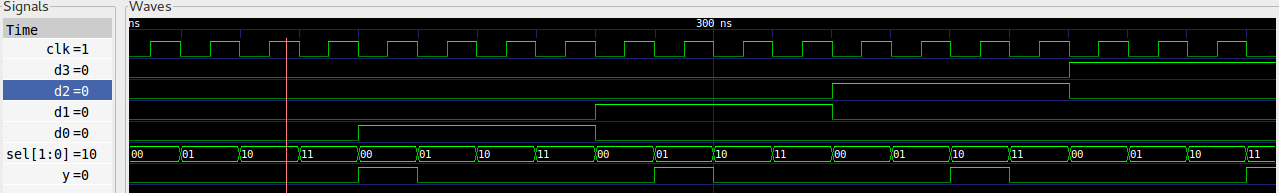
\includegraphics[width=1\columnwidth]{MUX_Sim}
\end{center}
\end{homeworkProblem}

\clearpage
%----------------------------------------------------------------------------------------

\end{document}